%!TEX root=../document.tex

\section{Ergebnisse}

\subsection{Möglichkeiten zur Datenhaltung}

\subsubsection{Websocket Implementation}
Es ist möglich eigene Server Nodes zu entwicklen, welche die Clients mithilfe von Websockets verwalten.


\subsubsection{Couchbase Mobile}
Couchbase Mobile ist eine Zusammensetzung aus Software, die eine NoSQL Datenbank darstellt und für Android und IOS Applikationen ausgelegt ist. Dies und die Synchronisation mit dem Couchbase Server und anderen Endgeräten erfolgt mit der Verwendung von Couchbase Lite und Couchbase Sync Gateway.

\subsubsection{Firebase}
Firebase ist eine Platform, welche von Google entwickelt wurde und viele Features für die Entwicklung von mobilen Applikationen bietet. Hauptsächlich auf Android und IOS. Außerdem bietet es Features zur Überwachung und Analyse der Datenbanken.

\section{Umsetzung}
Als Hilfe bei der Umsetzung der mobilen Applikation wurde ein Tutorial hergenommen. Da mit diesem aber keine Einkaufsliste erstellt wird, musste diese Applikation noch etwas abgeändert werden. \\
\href{http://www.appsdeveloperblog.com/todo-list-app-kotlin-firebase/}{http://www.appsdeveloperblog.com/todo-list-app-kotlin-firebase/}

\subsection{Verwendete Programmiersprache}
Bei der Auswahl der Programmiersprache wurde sich an das Tutorial gehalten. Es wurde die Programmiersprache Kotlin verwendet. \\
Kotlin ist eine statisch typisierte Programmiersprache, welche für die JVM (Java Virtual Machine) übersetzt wird. Der Bytecode kann auch in JavaScript Quellcode umgewandelt werden. Kotlin wird von dem JetBrains Programmierern weiterentwickelt.

\subsection{Verwendete Datenhaltungsmöglichkeit}
Entschieden wurde sich für Firebase, da es eine der \glqq stärksten\grqq \ Echtzeit Datenbanken-API ist. Außerdem ist die Anbindung an eine Firebase Datenbank in Android Studio um einiges unumständlicher als bei z.B.: Couchbase.

\clearpage

\subsection{Projekt aufsetzen}
Entwickelt wurde mit der Entwicklungsumgebung \textbf{Android-Studio}. Wenn Android Studio gestartet wurde, wird zuerst ein neues Projekt erstellt. Hierbei ist wichtig, dass ein Häkchen bei \textbf{Include Kotlin support} gesetzt wird bevor das Projekt erstellt wird.

\begin{figure}[!h]
	\begin{center}
		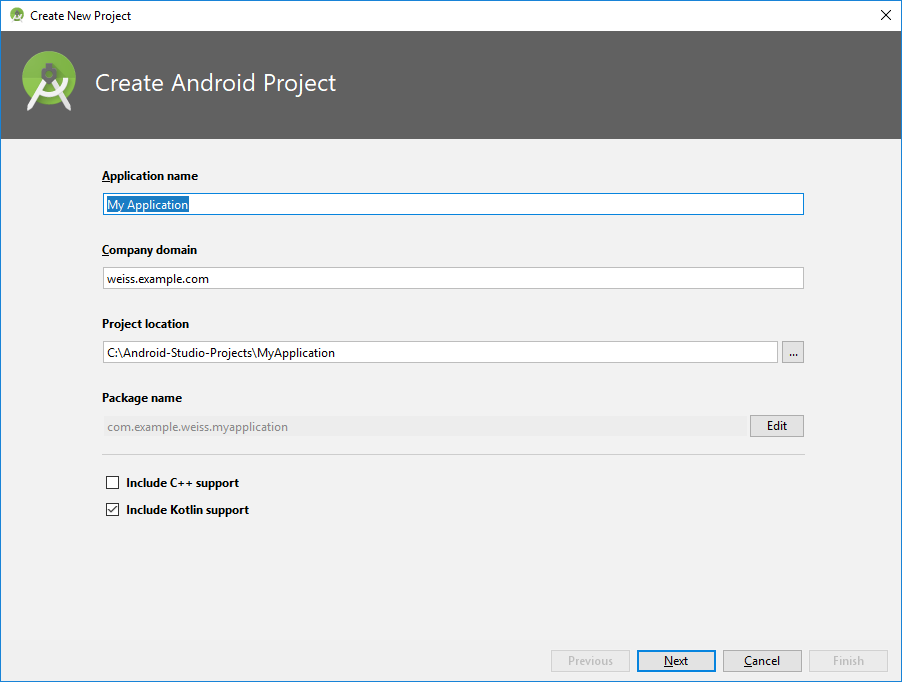
\includegraphics[width=0.6\linewidth]{images/proj-erst.png}
		\caption{Projekt erstellen}
	\end{center}
\end{figure}

Wenn das Projekt erstellt wurde, wird als nächstes die Firebase Unterstützung hinzugefügt. Hierzu muss oben in der \textbf{Toolbar} auf \textbf{Tools > Firebase} geklickt werden.

\begin{figure}[!h]
	\begin{center}
		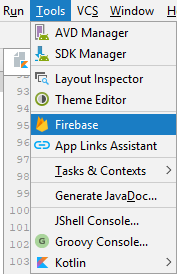
\includegraphics[width=0.2\linewidth]{images/firebase-supp.png}
		\caption{Firebase Support}
	\end{center}
\end{figure}

\clearpage

Dann erscheint auf der rechten Seite in Android Studio der Assisten für Firebase. Hier muss sich zur Datenbank verbunden werden, indem auf \textbf{Realtime Database} geklickt wird. Dort wird zur Datenbank verbunden und der Applikation kann die Datenbankverbindung hinzugefügt werden.

\begin{figure}[!h]
	\begin{center}
		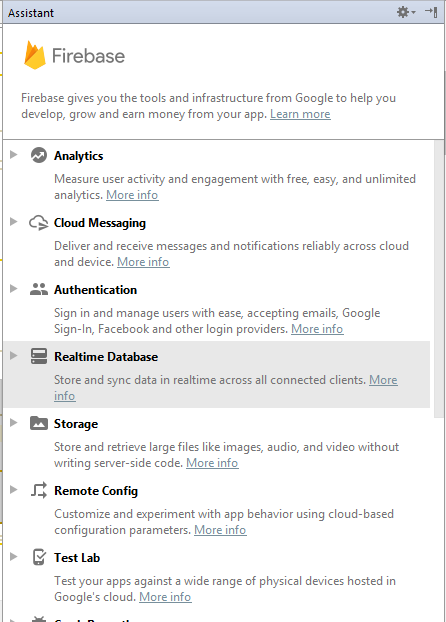
\includegraphics[width=0.5\linewidth]{images/firebase-ass.png}
		\caption{Firebase Assistent}
	\end{center}
\end{figure}

Wenn dies fertig ist, wird als nächstes auf der \textbf|Firebase Konsole| im Browser unter dem Reiter \textbf{Develop > Database} eine Realtime Datenbank hinzugefügt und im \textbf{Testmodus} gestartet. Dieser Modus ermöglicht es jedem der die ID dieser Datenbank hat darauf zuzugreifen.

\begin{figure}[!h]
	\begin{center}
		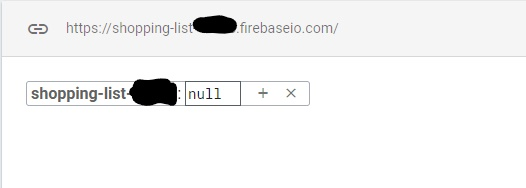
\includegraphics[width=0.6\linewidth]{images/database.jpg}
		\caption{Datenbank im Browser}
	\end{center}
\end{figure}

\clearpage

Nun kann mit der Implementierung begonnen werden. Zuerst wird eine Kotlin Datei erstellt, damit der Firebase Datenbank eine Collection hinzugefügt wird. Diese wird shop-item genannt.

\begin{lstlisting}
object Constants {
	@JvmStatic val FIREBASE_ITEM: String = "shop_item"
}
\end{lstlisting}

In der selben Datei wird auch noch ein Model für ein \textbf{ShopItem} erstellt. Dies ist eine Klasse in der eine Objekt-ID, ein Text als Beschreibung und eine Boolean Variable, welche verwendet wird um zu überprüfen ob dieses Item angehakelt wurde.

\begin{lstlisting}
class ShopItem {
	companion object Factory {
		fun create(): ShopItem = ShopItem()
	}
	var objectId: String? = null
	var itemText: String? = null
	var done: Boolean? = false
}
\end{lstlisting}

Dann wird die App designed. Dies ist jedem selbst überlassen wie diese aussieht. Funktionalitäten, welche der App hinzugefügt wurden.
\begin{itemize}
	\item ein \textbf|FloatingButton|, welcher ein Dialog Fenster öffnet um Items hinzuzufügen
	\item eine \textbf{ListView} und eine \textbf{Checkbox} in jeder Reihe
	\item wenn die Checkbox geklickt wird, dann wird diese als \glqq Fertig\grqq \ angezeigt
	\item ebenfalls in jeder Reihe ein \textbf{DeleteButton}, um die Einträge wieder heraus zu löschen
\end{itemize}

\clearpage

Diese sieht dann ungefähr wie folgt aus:

\begin{figure}[!h]
	\begin{center}
		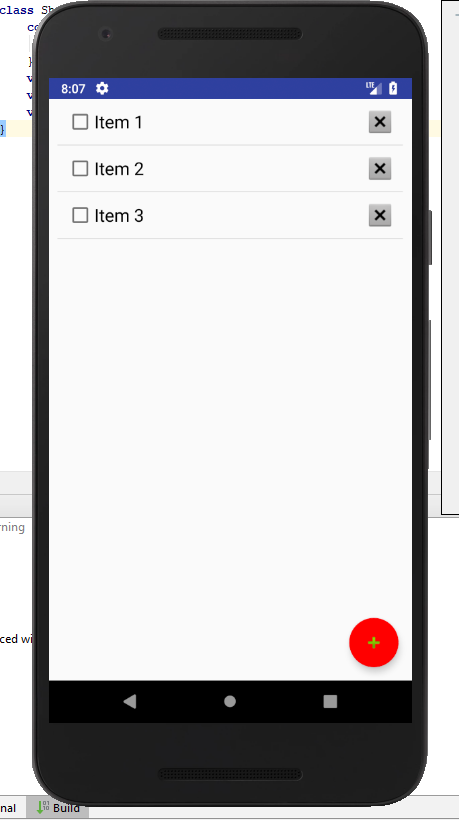
\includegraphics[width=0.4\linewidth]{images/app-design.png}
		\caption{Design der App}
	\end{center}
\end{figure}

\subsection{Dialog Fenster bei Button-Klick}
Diese Methode erstellt ein Dialog Fenster, in dem ein neues Item hinzugefügt werden kann. Weiters wird dem \textbf{Submit Button} die Funktion gegeben die neu eingegebenen Daten in die Firebase Datenbank zu speichern, dies geschieht mit \textbf{.push()}. 

\begin{lstlisting}
private fun addNewItemDialog() {
	val alert = AlertDialog.Builder(this)
	val itemEditText = EditText(this)
	alert.setMessage("Add New Item")
	alert.setTitle("Enter To Do Item Text")
	alert.setView(itemEditText)
	alert.setPositiveButton("Submit") { dialog, positiveButton ->
		val shopItem = ShopItem.create()
		shopItem.itemText = itemEditText.text.toString()
		shopItem.done = false
		val newItem = mDatabase.child(Constants.FIREBASE_ITEM).push()
		shopItem.objectId = newItem.key
		newItem.setValue(shopItem)
		dialog.dismiss()
		Toast.makeText(this, "Item saved with ID " + shopItem.objectId, Toast.LENGTH_SHORT).show()
	}
	alert.show()
}
\end{lstlisting}

Wenn man die Datenbank im Browser aufruft, werden jetzt alle hinzugefügten Daten angezeigt.

\begin{figure}[!h]
	\begin{center}
		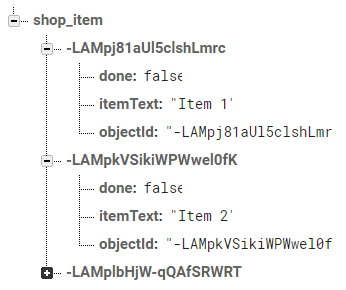
\includegraphics[width=0.5\linewidth]{images/database-entry.png}
		\caption{Daten in der Datenbank}
	\end{center}
\end{figure}

\subsection{Daten in Liste einfügen}
Die folgende Methode wird dafür verwendet um in der App alle Einträge in einer Liste darzustellen. Dafür werden alle Daten aus der Datenbank ausgelesen und nacheinander in die Liste der App eingefügt. Hier muss aber vor dem Einfügen aller Daten die Liste in der App nochmals \glqq gecleared\grqq \ (\textbf{.clear()}) werden, ansonsten würden alle Daten öfters in die Liste eingetragen werden.


\begin{lstlisting}
private fun addDataToList(dataSnapshot: DataSnapshot) {
	val items = dataSnapshot.children.iterator()
	shopList!!.clear();
	if (items.hasNext()) {
		val shopListindex = items.next()
		val itemsIterator = shopListindex.children.iterator()

		while (itemsIterator.hasNext()) {
			val currentItem = itemsIterator.next()
			val shopItem = ShopItem.create()
			val map = currentItem.getValue() as HashMap<String, Any>
			shopItem.objectId = currentItem.key
			shopItem.done = map.get("done") as Boolean?
			shopItem.itemText = map.get("itemText") as String?
			shopList!!.add(shopItem);
		}
	}
	adapter.notifyDataSetChanged()
}
\end{lstlisting}

\clearpage

\subsection{Daten checken}
Mit einem Klick auf die Checkbox wird diese \glqq aktiviert\grqq \ und der Boolean wert in der Datenbank wird verändert, damit auf allen Geräten die Checkbox geändert wird.

\begin{lstlisting}
override fun modifyItemState(itemObjectId: String, isDone: Boolean) {
	val itemReference = mDatabase.child(Constants.FIREBASE_ITEM).child(itemObjectId)
	itemReference.child("done").setValue(isDone);
}
\end{lstlisting}

\subsection{Daten löschen}
Ein Klick auf den \textbf{Löschen Button} löscht den Eintrag aus der Liste und aus der Datenbank, damit auch auf allen anderen Geräten dieser Eintrag nicht mehr angezeigt wird.

\begin{lstlisting}
override fun onItemDelete(itemObjectId: String) {
	val itemReference = mDatabase.child(Constants.FIREBASE_ITEM).child(itemObjectId)
	itemReference.removeValue()
}
\end{lstlisting}

\subsection{Firebase Offline Persisting}
Firebase kann Daten sehr einfach und schnell \textbf{cachen}. Firebase wird die Daten der Datenbank auf deinem Gerät zu cachen und wenn die App wieder Online geht, dann werden die Daten mit der Datenbank abgeglichen und aktualisiert.
\\ Hierzu wird eine Application Klasse erstellt in der diese Funktionalität aktiviert wird.

\begin{lstlisting}
class ThisApplication: Application() {
	override fun onCreate() {
		super.onCreate()
		FirebaseDatabase.getInstance().setPersistenceEnabled(true)
	}
}
\end{lstlisting}



\clearpage